\chapter{Badania}
\label{chapter:research}

W rozdziale tym zostały zaprezentowane wyniki badań przeprowadzone dla przykładowych funkcji referencyjnych.
Wszystkie funkcje opisane w tym rozdziale,
ale nie załączone bezpośrednio,
znajdują się w załącznikach niniejszej pracy dyplomowej.

\section{Filtr f5}

Przykładem potwierdzającym skuteczność algorytmu opracowanego w ramach niniejszej pracy
może być układ arytmetyki rozproszonej \cite{memory-capacity} filtru f5 \cite{nine-filters}.
Reprezentacja tego układu za pomocą w pełni określonych funkcji boolowskich
jest opisana tablicą o 11 zmiennych wejściowych i 11 wyjściach.
Implementacja tego układu \cite{redukcja-kompresja} w strukturze Virtex-7 wykonana za pomocą programu Vivado 2015.4.2
wymaga zastosowania 531 komórek (330 6-wejściowych, 86 5-wejściowych; pozostałe 4, 3 i 2-wejściowe).
Opracowany algorytm redukcji i kompresji argumentów (dalej nazywany algorytmem RedKomp)
redukuje tę funkcję do 7 argumentów,
umożliwiając jej realizację
(wykonywana w tej samej strukturze programem Vivado)
w strukturze zajmującej 9 komórek 6-wejściowych oraz po jednej 5, 4 i 2-wejściowej.

\section{Przykład Sasao}

Eksperyment opisany w tym rozdziale dotyczy generatora indeksów analizowanego w referacie Sasao \cite{sasao-workshop}.
Dla funkcji przedstawionej w tableli \ref{sasao-a} profesor Sasao wyznaczył 5-argumentowy redukt – tabela \ref{sasao-b}.
Dzięki zastosowaniu program RedKomp udało się ten wynik poprawić uzyskując redukt 4-argumentowy,
przedstawiony w tabeli \ref{sasao-c}.

\begin{table}[t]
\caption{Przykład funkcji generatora indeksów Sasao \cite{sasao-workshop}}
\begin{subtable}{.64\linewidth}
\caption{Pełna wersja}
\label{sasao-a}
\begin{tabular}{|r@{}c@{}c@{}c@{}c@{}c@{}c@{}c@{}c@{}c@{}c@{}c@{}c@{}c@{}c@{}c@{}c@{}c@{}c@{}c@{}c@{}c@{}c@{}c@{}c@{}c@{}c@{}c@{}c@{}c@{}c@{}c@{}c@{}c@{}c@{}c@{}c@{}c@{}c@{}c|l|}
\hline
0 & 1 & 1 & 0 & 0 & 0 & 0 & 1 & 0 & 0 & 0 & 1 & 0 & 0 & 0 & 0 & 1 & 0 & 1 & 0 & 0 & 1 & 1 & 0 & 0 & 0 & 0 & 1 & 0 & 0 & 0 & 1 & 0 & 0 & 0 & 0 & 1 & 0 & 1 & 0   &   1 \\
0 & 1 & 0 & 1 & 1 & 1 & 1 & 1 & 0 & 1 & 1 & 0 & 1 & 0 & 1 & 0 & 0 & 0 & 1 & 1 & 0 & 1 & 0 & 1 & 1 & 1 & 1 & 1 & 0 & 1 & 1 & 0 & 1 & 0 & 1 & 0 & 0 & 0 & 1 & 1   &   2 \\
1 & 1 & 1 & 1 & 0 & 1 & 0 & 1 & 0 & 1 & 1 & 1 & 0 & 1 & 1 & 1 & 0 & 0 & 0 & 0 & 1 & 1 & 1 & 1 & 0 & 1 & 0 & 1 & 0 & 1 & 1 & 1 & 0 & 1 & 1 & 1 & 0 & 0 & 0 & 1   &   3 \\
0 & 0 & 0 & 1 & 1 & 1 & 1 & 0 & 0 & 0 & 0 & 1 & 0 & 0 & 0 & 1 & 0 & 1 & 1 & 1 & 0 & 0 & 0 & 1 & 1 & 1 & 1 & 0 & 0 & 0 & 0 & 1 & 0 & 0 & 0 & 1 & 0 & 1 & 1 & 1   &   4 \\
0 & 0 & 1 & 1 & 1 & 1 & 0 & 0 & 0 & 0 & 0 & 0 & 0 & 1 & 0 & 0 & 0 & 1 & 0 & 1 & 0 & 0 & 1 & 1 & 1 & 1 & 0 & 0 & 0 & 0 & 0 & 0 & 0 & 1 & 0 & 0 & 0 & 1 & 0 & 1   &   5 \\
0 & 1 & 1 & 1 & 0 & 0 & 1 & 0 & 0 & 1 & 0 & 0 & 0 & 1 & 0 & 0 & 1 & 0 & 0 & 1 & 0 & 1 & 1 & 1 & 0 & 0 & 1 & 0 & 0 & 1 & 0 & 0 & 0 & 1 & 0 & 0 & 1 & 0 & 0 & 1   &   6 \\
0 & 0 & 1 & 0 & 0 & 0 & 1 & 1 & 1 & 0 & 0 & 0 & 1 & 1 & 1 & 1 & 0 & 0 & 1 & 0 & 0 & 0 & 1 & 0 & 0 & 0 & 1 & 1 & 1 & 0 & 0 & 0 & 1 & 1 & 1 & 1 & 0 & 0 & 1 & 0   &   7 \\
1 & 1 & 1 & 1 & 1 & 1 & 1 & 1 & 1 & 1 & 0 & 1 & 0 & 0 & 0 & 1 & 1 & 1 & 1 & 0 & 0 & 0 & 1 & 0 & 0 & 0 & 1 & 1 & 1 & 0 & 0 & 0 & 1 & 1 & 1 & 1 & 0 & 0 & 1 & 0   &   8 \\
1 & 1 & 1 & 0 & 1 & 1 & 1 & 0 & 0 & 0 & 1 & 1 & 0 & 0 & 0 & 1 & 0 & 1 & 1 & 0 & 1 & 1 & 1 & 0 & 1 & 1 & 1 & 0 & 0 & 0 & 1 & 1 & 0 & 0 & 0 & 1 & 0 & 1 & 1 & 0   &   9 \\
1 & 0 & 1 & 0 & 0 & 0 & 0 & 1 & 1 & 0 & 1 & 0 & 0 & 1 & 0 & 0 & 0 & 0 & 1 & 1 & 1 & 0 & 1 & 0 & 0 & 0 & 0 & 1 & 1 & 0 & 1 & 0 & 0 & 1 & 0 & 0 & 0 & 0 & 1 & 1   &   10 \\
\hline
\end{tabular}
\end{subtable}
\begin{subtable}{.12\linewidth}
\caption{Sasao}
\label{sasao-b}
\begin{tabular}{|r@{}c@{}c@{}c@{}l|}
\hline
0 & 1 & 1 & 0 & 0 \\
0 & 1 & 0 & 1 & 1 \\
1 & 1 & 1 & 1 & 1 \\
0 & 0 & 0 & 1 & 1 \\
0 & 0 & 1 & 1 & 1 \\
0 & 1 & 1 & 1 & 1 \\
0 & 0 & 1 & 0 & 0 \\
1 & 1 & 1 & 1 & 0 \\
1 & 1 & 1 & 0 & 0 \\
1 & 0 & 1 & 0 & 1 \\
\hline
\end{tabular}
\end{subtable}
\begin{subtable}{.16\linewidth}
\caption{RedKomp}
\label{sasao-c}
\begin{tabular}{|r@{}c@{}c@{}l|}
\hline
1 & 0 & 0 & 0 \\
0 & 0 & 0 & 0 \\
1 & 0 & 1 & 0 \\
0 & 0 & 1 & 0 \\
1 & 1 & 0 & 0 \\
1 & 1 & 1 & 1 \\
0 & 0 & 1 & 1 \\
0 & 1 & 0 & 0 \\
0 & 1 & 0 & 1 \\
0 & 0 & 0 & 1 \\
\hline
\end{tabular}
\end{subtable}
\end{table}

Rezultatem tego wyniku jest możliwość zrealizowania tej funkcji w strukturze zaproponowanej w referacie Sasao (rysunek \ref{fig:sasao-structure}) \cite{sasao-recent},
zbudowanej z dwóch pamięci: pamięć głównej i pomocniczej,
które mają zaledwie 4 wejścia adresowe.

\begin{figure}[H]
\centering
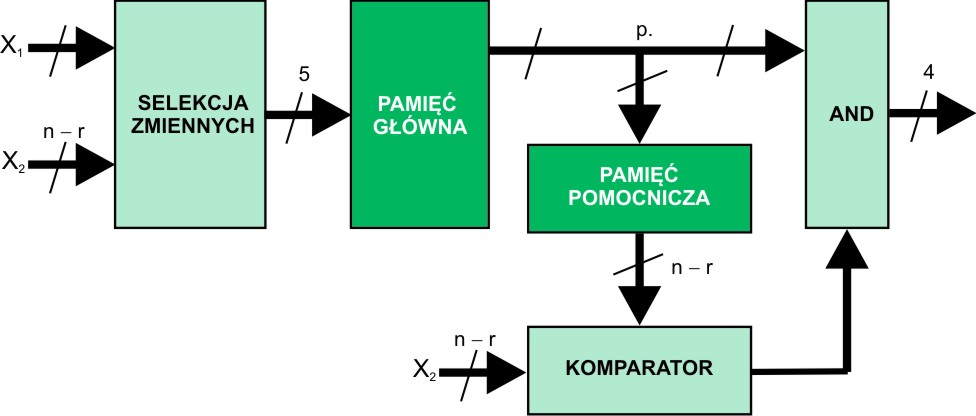
\includegraphics[width = 13cm]{chapter04/sasao-structure.jpg}
\caption{Strukturza zaproponowanej w referacie Sasao (źródło \cite{sasao-workshop}).}
\label{fig:sasao-structure}
\end{figure}

W~strukturze tej blok selekcji zmiennych wybiera spośród wszystkich zmiennych podzbiór $X_1$,
reprezentujący minimalną liczbę zmiennych realizowanej funkcji generowania indeksów.
Liczność reduktu jest r.
Jest to jednocześnie liczba wejść do pamięci głównej.
Na wyjściach pamięci głównej pojawia się indeks wektora wejściowego. % $X = X_1 \cup X_2$.
Jest on reprezentowany wektorem binarnym o liczbie bitów $p = \lceil log_2 (k+1)\rceil$.
Indeks ten jest poprawnym indeksem wektora wejściowego wtedy,
jeżeli jest to wektor rejestrowany.
I tylko wtedy indeks ten pojawi sie na wyjściach generatora.
W przypadku,
gdy wektor wejściowy nie jest wektorem rejestrowanym na wyjściach generator pojawi się 0.
Sprawdzenie,
czy wyjścia pamięci głównej reprezentują poprawny indeks jest realizowane w pamięci pomocniczej i komparatorze.
W pamięci pomocniczej są zapisane wektory reprezentowane zmiennymi należącymi do zbioru $X_2$.
Wektory te są podawane na wejście komparatora i porównywane z rzeczywistym wektorem $X_2$ podawanym na drugie wejście komparatora.
Oczywiście wektor pobrany z pamięci pomocniczej będzie różny od rzeczywistego wektora $X_2$ w przypadku,
gdy nie należy on do wektora rejestrowanego.
Wtedy komparator sygnałem wyjściowym 0 zablokuje pojawienie się na wyjściach bramy AND wektora wytworzonego w pamięci głównej.

\section{Permutacje 1 z 10}

Eksperyment opisany w tym rozdziale dotyczy funkcji ,,1 z 10'' (tabela \ref{1of10}) analizowanej w artykule \cite{sasao-s-min}.
Funkcja ta jest redukowalna do 9 zmiennych na wiele sposobów.
Jednym z nich jest usunięcie z funkcji nadmiarowego argumentu $x_2$.
Funkcję po usunięciu tego argumentu i zmianie oznaczeń na $a_1, ..., a_9$ przedstawiono w tabeli \ref(1of10-reduct)

\begin{table}[t]
\caption{Funkcja 1 z 10 \cite{sasao-s-min}.}
\label{1of10}
\begin{tabular}{|r|ccccc ccccc|ccc ccl|}
\hline
$F$ & $x_1$ & $x_2$ & $x_3$ & $x_4$ & $x_5$ & $x_6$ & $x_7$ & $x_8$ & $x_9$ & $x_{10}$ & $y_1$ & $y_2$ & $y_3$ & $y_4$ & $y_5$ & $y_6$ \\
\hline
1 & 1 & 0 & 0 & 0 & 0 & 0 & 0 & 0 & 0 & 0 & 1 & 0 & 0 & 0 & 0 & 0 \\
2 & 0 & 1 & 0 & 0 & 0 & 0 & 0 & 0 & 0 & 0 & 0 & 0 & 0 & 0 & 0 & 0 \\
3 & 0 & 0 & 1 & 0 & 0 & 0 & 0 & 0 & 0 & 0 & 0 & 1 & 1 & 0 & 0 & 0 \\
4 & 0 & 0 & 0 & 1 & 0 & 0 & 0 & 0 & 0 & 0 & 0 & 0 & 0 & 1 & 1 & 0 \\
5 & 0 & 0 & 0 & 0 & 1 & 0 & 0 & 0 & 0 & 0 & 0 & 0 & 0 & 0 & 0 & 1 \\
6 & 0 & 0 & 0 & 0 & 0 & 1 & 0 & 0 & 0 & 0 & 1 & 0 & 0 & 0 & 0 & 1 \\
7 & 0 & 0 & 0 & 0 & 0 & 0 & 1 & 0 & 0 & 0 & 0 & 1 & 0 & 0 & 0 & 0 \\
8 & 0 & 0 & 0 & 0 & 0 & 0 & 0 & 1 & 0 & 0 & 0 & 0 & 0 & 1 & 0 & 0 \\
9 & 0 & 0 & 0 & 0 & 0 & 0 & 0 & 0 & 1 & 0 & 0 & 0 & 1 & 0 & 0 & 0 \\
0 & 0 & 0 & 0 & 0 & 0 & 0 & 0 & 0 & 0 & 1 & 0 & 0 & 0 & 0 & 1 & 0 \\
\hline
\end{tabular}
\end{table}
\begin{table}[H]
\caption{Optymalizowana funkcja ,,1 z~10'' \cite{sasao-s-min}.}
\begin{subtable}{.64\linewidth}
\caption{Po redukcji}
\label{1of10-reduct}

\begin{tabular}{|r|c@{}c@{}c@{}c@{}c@{}c@{}c@{}c@{}c|c@{}c@{}c@{}c@{}c@{}l|}
\hline
$F$ & $a_1$ & $a_2$ & $a_3$ & $a_4$ & $a_5$ & $a_6$ & $a_7$ & $a_8$ & $a_9$ & $y_1$ & $y_2$ & $y_3$ & $y_4$ & $y_5$ & $y_6$ \\
\hline
1 & 1 & 0 & 0 & 0 & 0 & 0 & 0 & 0 & 0 & 1 & 0 & 0 & 0 & 0 & 0 \\
2 & 0 & 0 & 0 & 0 & 0 & 0 & 0 & 0 & 0 & 0 & 0 & 0 & 0 & 0 & 0 \\
3 & 0 & 1 & 0 & 0 & 0 & 0 & 0 & 0 & 0 & 0 & 1 & 1 & 0 & 0 & 0 \\
4 & 0 & 0 & 1 & 0 & 0 & 0 & 0 & 0 & 0 & 0 & 0 & 0 & 1 & 1 & 0 \\
5 & 0 & 0 & 0 & 1 & 0 & 0 & 0 & 0 & 0 & 0 & 0 & 0 & 0 & 0 & 1 \\
6 & 0 & 0 & 0 & 0 & 1 & 0 & 0 & 0 & 0 & 1 & 0 & 0 & 0 & 0 & 1 \\
7 & 0 & 0 & 0 & 0 & 0 & 1 & 0 & 0 & 0 & 0 & 1 & 0 & 0 & 0 & 0 \\
8 & 0 & 0 & 0 & 0 & 0 & 0 & 1 & 0 & 0 & 0 & 0 & 0 & 1 & 0 & 0 \\
9 & 0 & 0 & 0 & 0 & 0 & 0 & 0 & 1 & 0 & 0 & 0 & 1 & 0 & 0 & 0 \\
0 & 0 & 0 & 0 & 0 & 0 & 0 & 0 & 0 & 1 & 0 & 0 & 0 & 0 & 1 & 0 \\
\hline
\end{tabular}

\end{subtable}
\begin{subtable}{.12\linewidth}
\caption{Sasao}
\label{1of10-reduct-b}

\begin{tabular}{|r@{}c@{}c@{}c@{}l|}
\hline
  &   &   &   &   \\
\hline
1 & 0 & 0 & 0 & 0 \\
0 & 0 & 0 & 0 & 0 \\
0 & 1 & 1 & 0 & 1 \\
0 & 0 & 1 & 1 & 0 \\
0 & 0 & 0 & 0 & 1 \\
1 & 0 & 0 & 0 & 1 \\
0 & 1 & 0 & 0 & 0 \\
0 & 0 & 0 & 1 & 0 \\
0 & 0 & 1 & 0 & 1 \\
0 & 0 & 1 & 0 & 0 \\
\hline
\end{tabular}

\end{subtable}
\begin{subtable}{.16\linewidth}
\caption{RedKomp}
\label{1of10-reduct-c}

\begin{tabular}{|r@{}c@{}c@{}l|}
\hline
$b_1$ & $b_2$ & $b_3$ & $b_4$ \\
\hline
1 & 0 & 0 & 0 \\
0 & 0 & 0 & 0 \\
1 & 0 & 1 & 0 \\
0 & 0 & 1 & 0 \\
1 & 1 & 0 & 0 \\
1 & 1 & 1 & 1 \\
0 & 0 & 1 & 1 \\
0 & 1 & 0 & 0 \\
0 & 1 & 0 & 1 \\
0 & 0 & 0 & 1 \\
\hline
\end{tabular}

\end{subtable}
\end{table}


Przy tych oznaczeniach Sasao, stosując algorytm 2-Min obliczył dekompozycję \cite{sasao-s-min}:

Następnie po zastosowaniu algorytmu 3-Min indeksowanie zostało poprawione do wektorów 5-bitowych \cite{sasao-s-min}:

Rezultat uzyskany metodą RedKomp jest 4-bitowy (patrz Dodatek):

\section{Permutacje 2 z 16}

Eksperyment opisany w tym rozdziale dotyczy funkcji ,,2 z 16''.
Dekompozycja liniowa tej funkcji obliczana algorytmem 2-Min oraz 3-Min \cite{sasao-s-min} tworzy układ o 11 wejściach.
Liczby wejść do poszczególnych bramek XOR nie są podane.
Program RedKomp umożliwia realizację tej funkcji na pamięci o 9 wejściach adresowych.
Poszczególne wejścia $y_1$ do $y_9$ tej pamięci są wyrażone następującymi funkcjami XOR:
\begin{multline} \\
y1 = x7 \oplus x1 \oplus x2, \\
y2 = x10 \oplus x2 \oplus x3, \\
y3 = x13 \oplus x6 \oplus x7, \\
y4 = x14 \oplus x9 \oplus x10, \\
y5 = x9 \oplus x10 \oplus x12 \oplus x13, \\
y6 = x0 \oplus x1 \oplus x3 \oplus x4, \\
y7 = x3 \oplus x4 \oplus x5 \oplus x6, \\
y8 = x5 \oplus x6 \oplus x8 \oplus x9, \\
y9 = x8 \oplus x9 \oplus x11 \oplus x12. \\
\end{multline}

\section{Permutacje 2 z 20}

Eksperyment opisany w tym rozdziale dotyczy funkcji ,,2 z 20''.
Dekompozycja liniowa tej funkcji obliczana algorytmem 2-Min oraz 3-Min \cite{sasao-s-min} tworzy układ o 14 wejściach.
Liczby wejść do poszczególnych bramek XOR nie są podane.
Program RedKomp umożliwia realizację tej funkcji na pamięci o 14 wejściach adresowych.
Poszczególne wejścia $y_1$ do $y_14$ tej pamięci są wyrażone następującymi funkcjami XOR:
\begin{multline} \\
y1 = x15, \\
y2 = x16, \\
y3 = x17, \\
y4 = x18, \\
y5 = x0 \oplus x1, \\
y6 = x3 \oplus x4, \\
y7 = x5 \oplus x6, \\
y8 = x7 \oplus x1 \oplus x2, \\
y9 = x8 \oplus x9, \\
y10 = x10 \oplus x2 \oplus x3, \\
y11 = x11 \oplus x12, \\
y12 = x13 \oplus x6 \oplus x7, \\
y13 = x14 \oplus x9 \oplus x10, \\
y14 = x9 \oplus x10 \oplus x12 \oplus x13. \\
\end{multline}

\section{Permutacje 2 z 20}

Eksperyment opisany w tym rozdziale dotyczy funkcji 2outof20.
Dekompozycja liniowa tej funkcji obliczana algorytmem 2-Min oraz 3-Min \cite{sasao-s-min} tworzy układ o 14 wejściach.
Program RedKomp umożliwia realizację tej funkcji na pamięci o 9 wejściach adresowych.
Poszczególne wejścia $y_1$ do $y_9$ tej pamięci są następującymi funkcjami XOR:

\begin{multline} \\
y1 = x3 \oplus x4 \oplus x9 \oplus x10 \oplus x12 \oplus x13, \\
y2 = x10 \oplus x2 \oplus x3 \oplus x15 \oplus x16, \\
y3 = x15 \oplus x16 \oplus x18 \oplus x0 \oplus x1, \\
y4 = x13 \oplus x6 \oplus x7 \oplus x14 \oplus x9 \oplus x10, \\
y5 = x14 \oplus x9 \oplus x10 \oplus x17 \oplus x7 \oplus x1 \oplus x2, \\
y6 = x17 \oplus x7 \oplus x1 \oplus x2 \oplus x0 \oplus x1 \oplus x3 \oplus x4, \\
y7 = x0 \oplus x1 \oplus x3 \oplus x4 \oplus x8 \oplus x9 \oplus x11 \oplus x12, \\
y8 = x8 \oplus x9 \oplus x11 \oplus x12 \oplus x11 \oplus x12 \oplus x16 \oplus x17, \\
y9 = x11 \oplus x12 \oplus x16 \oplus x17 \oplus x18 \oplus x0 \oplus x1 \oplus x5 \oplus x6 \oplus x8 \oplus x9. \\
\end{multline} \\

Z eksperymentów 5 i 6 wynika, że program RedKomp ma większe możliwości.
Potrafi skuteczniej redukować wejścia do pamięci ROM,
a w szczególności potrafi zmniejszać liczbę wejść do pamięci
kosztem zwiększania liczby wejść do poszczególnych bramek XOR.
Nadmierna liczba wejść do bramek XOR nie będzie nigdy problemem.
Wielowejściową bramkę XOR niedostępną w układzie ze względu na liczbę wejść,
zawsze można zastąpić kilkoma mniejszymi bramkami stosując strukturę wielopoziomową.